\documentclass[10pt,a4paper]{article}
\usepackage[utf8]{inputenc}
\usepackage[italian]{babel}
\usepackage{amsmath}
\usepackage{amsfonts}
\usepackage{amssymb}
\usepackage{graphicx}
\usepackage[left=2cm,right=2cm,top=2cm,bottom=2cm]{geometry}
\newcommand{\rem}[1]{[\emph{#1}]}

\author{Gruppo xx \\ Mario Rossi, Anna Bianchi \rem{non dimenticate i nomi}}
\title{Esercitazione N.1: Misure di tensione, corrente, tempi, frequenza.}
\begin{document}

\maketitle

\section{Scopo e strumentazione}

L'esercitazione ha lo scopo di impratichirsi con la strumentazione e le tecniche di misura. 
Abbiamo utilizzato sia il multimetro digitale sia il tester analogico. 

\section{Misure di tensione e corrente}
\paragraph{2.b Partitore}
Abbiamo montato il circuito in Fig. 1 con i valori di resistenza misurati con il multimetro digitale: $R_1 = 1.12\pm 0.01 k\Omega$ e $R_2 = 0.95\pm 0.01 k\Omega$. L'errore \`e stato stimato usando le indicazioni del manuale del multimetro ($0.8\%$ + 1 cifra). 
Dall'analisi del circuito ci aspettiamo che $V_\mathrm{OUT}/V_\mathrm{IN} = \frac{1}{1+R_1/R_2}= 0.459 \pm 0.003 $.

\rem{Nota sul calcolo di questo errore: l'errore relativo sul rapporto delle resistenze \`e 1.4\%. Poich\`e il rapporto \`e circa 1, l'errore assoluto \`e 0.014. Quando sommo 1 (numero puro) l'errore assoluto rimane lo stesso ma quello relativo diventa 0.014/2= 0.7\%. Facendo l'inverso l'errore relativo rimane lo stesso, per cui l'errore finale sul rapporto \`e 0.7\% * 0.459 = 0.003}

Variando $V_\mathrm{IN}$ tra 0 e 10V abbiamo ottenuto i dati riportati in Tabella~\ref{t:par1} e Figura~\ref{f:par1}.

\begin{table}[h]
\centering
\begin{tabular}{|c|c|c|c|c|c|}
\hline 
VIN& $\sigma$ VIN  &VOUT	 & $\sigma$ VOUT& VOUT/VIN & $\sigma$ VOUT/VIN \\
\hline 
1.01&0.01&0.465&0.005&0.460&0.006\\
2.02&0.02&0.93&0.01&0.460&0.006\\
2.99&0.03&1.35&0.01&0.452&0.006\\
3.95&0.04&1.83&0.02&0.463&0.006\\
5.01&0.05&2.27&0.02&0.453&0.006\\
7.50&0.08&3.4&0.03&0.453&0.006\\
10.02&0.10&4.55&0.05&0.454&0.006\\
\hline 
\end{tabular} 
\caption{Partitore di tensione con resistenze da circa 1k. Tutte le tensioni in V.\label{t:par1}}
\end{table}
\begin{figure}
\centering
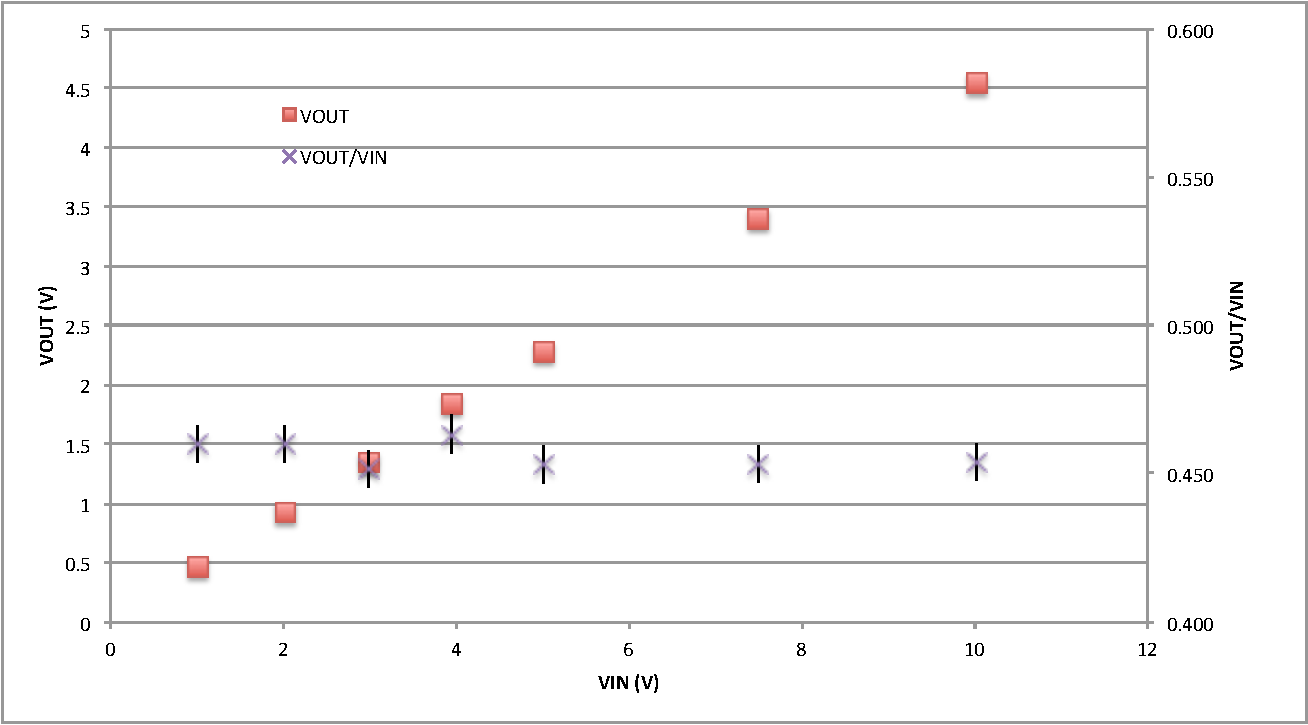
\includegraphics[scale=0.4]{part1.pdf}
\caption{Partitore di tensione.\label{f:par1}}
\end{figure}
Come ci si aspettava la relazione tra tensione di ingresso ed uscita \`e lineare. Il rapporto VOUT/VIN \`e da confrontare con il valore aspettato indicato sopra.

\rem{Volendo si pu\`o fare la media pesata dei valori misurati }

\paragraph{2.c Partitore con resitenze pi\`u grandi}
Montando di nuovo il partitore con le resistenze $R_1 = 3.80\pm 0.04 M\Omega$ e $R_2 = 3.95\pm 0.04 M\Omega$ si osservano i nuovi dati in Tabella~\ref{t:par2} e Figura~\ref{f:par2}
\begin{table}[h]
\centering
\begin{tabular}{|c|c|c|c|c|c|}
\hline 
VIN& $\sigma$ VIN  &VOUT	 & $\sigma$ VOUT& VOUT/VIN & $\sigma$ VOUT/VIN \\
\hline 
1.01&0.01&0.43&0.004&0.426&0.006\\
2.02&0.02&0.87&0.01&0.431&0.006\\
2.99&0.03&1.26&0.01&0.421&0.006\\
3.95&0.04&1.68665&0.02&0.427&0.006\\
5.01&0.05&2.13927&0.02&0.427&0.006\\
7.5&0.08&3.2025&0.03&0.427&0.006\\
10.02&0.10&4.27854&0.04&0.427&0.006\\
\hline 
\end{tabular} 
\caption{Partitore di tensione. Tutte le tensioni in V.\label{t:par2}}
\end{table}
\begin{figure}
\centering
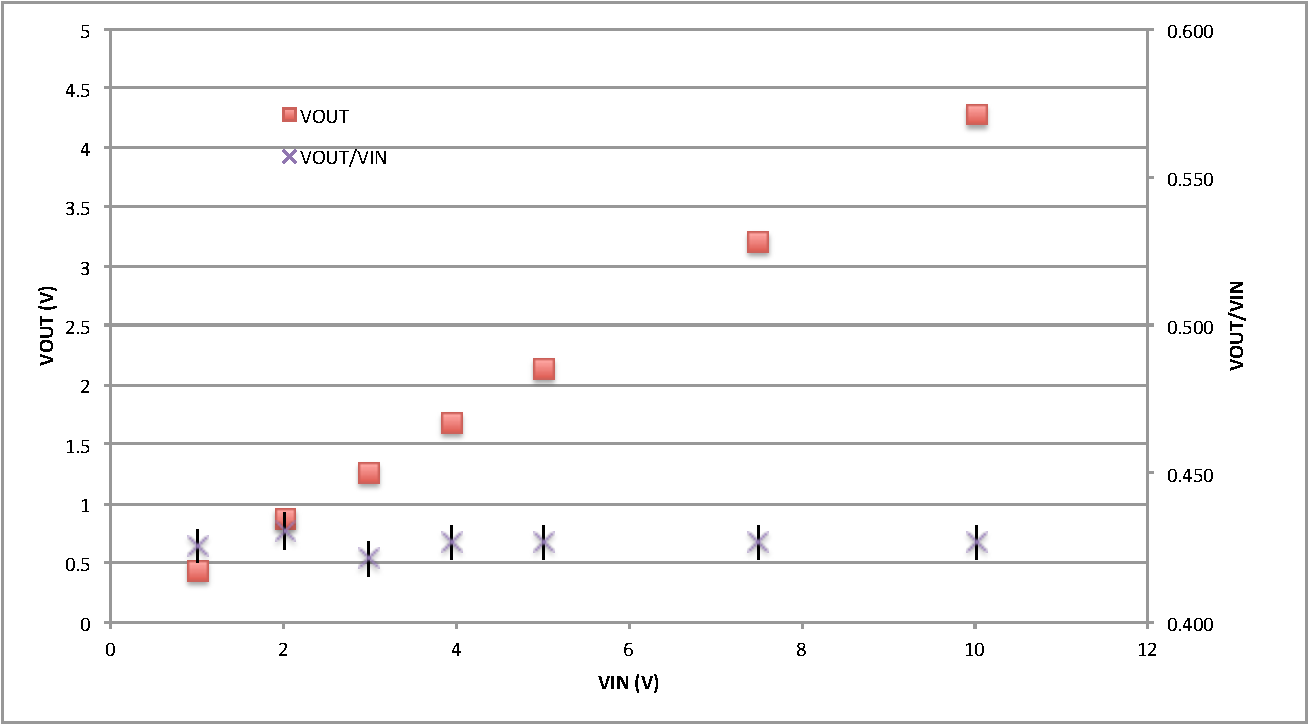
\includegraphics[scale=0.4]{part2.pdf}
\caption{Partitore di tensione con resistenze da circa 1M.\label{f:par2}}
\end{figure}

Si osserva come valore del rapporto misurato con le resistenze da $4~M\Omega$ si discosti da quanto atteso   $V_\mathrm{OUT}/V_\mathrm{IN} = \frac{1}{1+R_1/R_2}= 0.510\pm 0.003 $. La ragione della discrepanza \`e da ricercarsi nella impedenza di ingresso del tester.


\paragraph{2.d Resistenza di ingresso del tester}

 Usando il modello mostrato nella scheda si ottiene
\[ \frac{R_1}{R_T} =  \frac{V_{IN}}{V_{OUT}} - (1 +  \frac{R_1}{R_2} )
\]
L'errore sul secondo membro \`e: 1.4\% sul primo termine, 0.7\% sul secondo termine. Entrambi i termini sono circa 2, per cui l'errore totale \`e $ 0.03 \oplus 0.015 = 0.035$, dominato dalla misura di tensione. Quindi se  $R_T > R_1/0.035 $ non abbiamo nessuna sensibilit\`a sperimentale. 
Nel primo caso risulta un numero compatibile con 0: usando VIN = 5V abbiamo $R_1/R_T =0.027 \pm 0.035 $.
Nel secondo caso risulta invece $R_1/R_T =0.38 \pm 0.035 $ cio\`e $ R_T = 10 \pm 0.9 M\Omega$.

\subsection{Partitore di corrente: 2.e}

Si monta il circuito indicato con i valori di resistenza misurati con il multimetro digitale: 
$R_3= 105\pm 2 k\Omega$, $R_1 = 550\pm 5 \Omega$, $R_2 = 230\pm 3 \Omega$.
Si fissa la tensione dell'alimentatore a $V_{IN}=10.2 \pm 0.1 V$ e si utilizza il tester digitale per misurare alternativamente la corrente nel ramo 1 e nel ramo 2, sostitendo il ramo non sotto misura con un cortocircuito. 

\rem{NOTA BENE: nelle misure di corrente \`e importante prima fare le connessioni e poi accendere l'alimentatore, per cui bisogna sempre spegnere l'alimentatore prima di modificare le connessioni.}

Si ottengono le seguenti misure: $I1 = xx \pm y \mu ~A $, $I2 = xx \pm y \mu ~A $. 
Si ripetono le misure utilizzando il tester analogico, e si ottengono i seguenti valori:
$I1 = xx \pm y \mu A $, $I2 = xx \pm y \mu ~A $. 
Ci si aspetterebbe che il rapporto tra le correnti sia $I1/I2 = R2/R1 = 0.418 \pm 0.006$ e che la somma delle correnti sia $I1 + I2 = I_{TOT} \equiv V_{IN}/R3 = 97 \pm 2 \mu~A$, considerando che l'approssimazione $I_{TOT}=V_{IN}/R3$ vale quando $R3>>$altre resistenze in gioco, ed \`e certamente verificata in questo circuito. 
Tuttavia si nota che i valori effettivamente misurati con il tester analogico ed il tester digitale si discostano da tali valori:

\begin{center}
\begin{tabular}{|c|c|c|c|c|c|c|c|c|}
\hline 
strumento& I1 ($\mu A$)& $\sigma$(I1) ($\mu A$) & I2	($\mu A$) & $\sigma$(I2) ($\mu A$) & I1/I2 
& $\sigma$(I1/I2) & I1+I2 & $\sigma$(I1+I2) \\
\hline 
Analogico & xx & xx  & xx & xx & xx & xx & xx & xx \\
Digitale & xx & xx  & xx & xx & xx & xx & xx & xx \\
\hline 
\end{tabular} 
\end{center}

La discrepanza nasce dalla resistenza interna dell'amperometro che altera la 
resistenza lungo ciascun ramo quando viene inserito. Detta $R_A$ la resistenza dell'amperometro,
questa viene sommata alternativamente ad $R1$ oppure $R2$, per cui $I1/I2 = (R2+R_A)/(R1+R_A)$ 
e $I1+I2 = I_{TOT}\cdot(R1+R2)/(R1+R2+R_A)$.
Si pu\`o quindi stimare 
$$
R_A = (R1+R2)\left(\frac{I_{TOT}}{I1+I2} - 1 \right)
$$


\section{Uso dell'oscilloscopio}

\paragraph{Misure di tensione}

\paragraph{Impedenza di ingresso dell'oscilloscopio}

\section{Misure di frequenza e tempo}

\section{Trigger dell'oscilloscopio}

\section{Conclusioni e commenti finali}
Di questa esperienza non abbiamo capito molto, per\`o \`e stato divertente far saltare i fusibili. 


\end{document}